% !TeX root = ../main.tex
%
\chapter{Stabilization}
%
%\begin{figure}[H]
%  \hspace{-10pt}
%  \captionbox 
%  {
%    a
%    \label{fig:Edelta_twinSwingAndCatch}
%  }
%  {
%    \hspace{-1cm}
%    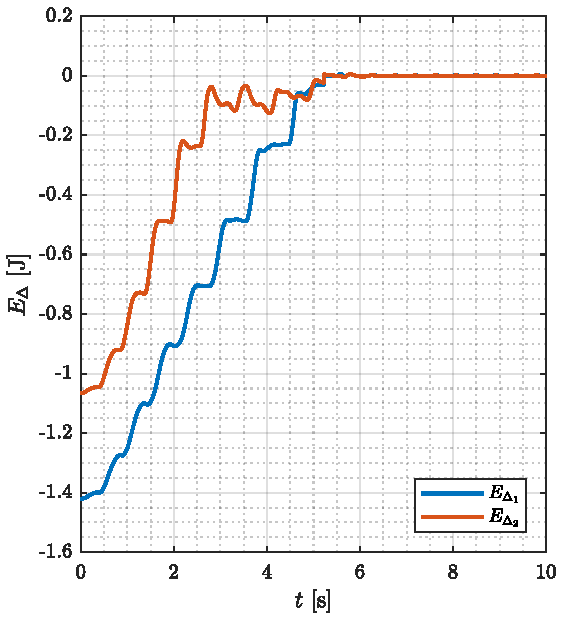
\includegraphics[width=.448\textwidth]{figures/Edelta_twinSwingAndCatch}
%  }
%  \hspace{20pt}
%  \captionbox 
%  {
%    a
%    \label{fig:phase_twinSwingAndCatch}
%  }
%  {
%    \hspace{-1cm}
%    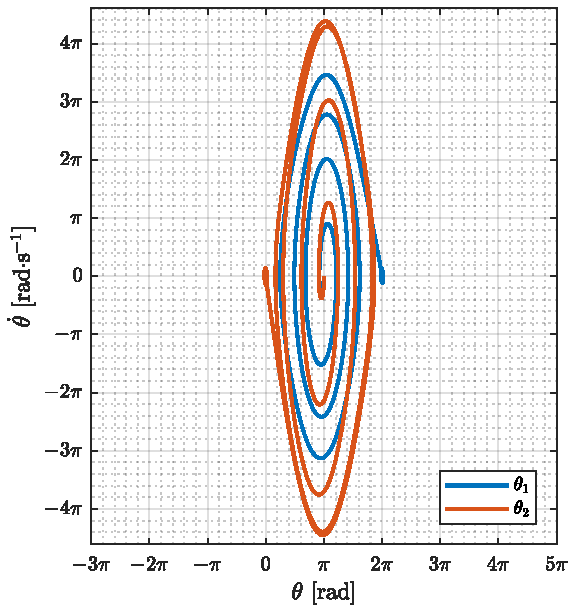
\includegraphics[width=.46\textwidth]{figures/phase_twinSwingAndCatch}
%  }
%\end{figure}
%
In this chapter a Linear Quadratic Regulator (LQR) is designed to stabilize the twin pendulum in upright position taking over from the swing-up controller. The design is based on \cite{triantafyllou2003maneuvering, franklin1994feedback} using the method described in \cite{lqrd}.\\
The nonlinear state space system from \autoref{eq:nonlinearStateSpaceTwin} is linearized,
\begin{align}
  \vec{A} &= \frac{\partial \vec{f(x)}}{\partial \vec{x}} \whereThree{\vec{x}=\vec{0}\ \ \ \ }{u=0\ \ \ \ }{\text{k}_\text{tanh}=1} \ \ \ , \ \ \
  \vec{B} = \frac{\partial \vec{f(x)}}{\partial u}  \whereThree{\vec{x}=\vec{0}\ \ \ \ }{u=0\ \ \ \ }{\text{k}_\text{tanh}=1} \ \ \ ,
  \label{eq:linearTwin_AB}
\end{align}
\begin{align}
  \vec{A} &= 
  \begin{bmatrix}
    0                         & 0                         & 0 & 1                                                    & 0                                                    & 0 \\
    0                         & 0                         & 0 & 0                                                    & 1                                                    & 0 \\
    0                         & 0                         & 0 & 0                                                    & 0                                                    & 1 \\
    \frac{g (M + m_1)}{M l_1} & \frac{g m_2}{M l_1}       & 0 & -\frac{(M + m_1)(b_{p_1,c} + b_{p_1,v})}{M l_1^2 m1} & -\frac{b_{p_2,c} + b_{p_2,v}}{M l_1 l_2}             & 0 \\
    \frac{g m_1}{M l_2}       & \frac{g (M + m_2)}{M l_2} & 0 & -\frac{b_{p_1,c} + b_{p_1,v}}{M l_1 l_2}             & -\frac{(M + m2)(b_{p_2,c} + b_{p_2,v})}{M l_2^2 m_2} & 0 \\
    \frac{g m_1}{M}           & \frac{g m_2}{M}           & 0 & -\frac{b_{p_1,c} + b_{p_1,v}}{M l_1}                 & -\frac{b_{p_2,c} + b_{p_2,v}}{M l_2}                 & 0
  \end{bmatrix}  \label{eq:linearTwin_A} \\
  \nonumber \\
  \vec{B} &= 
  \begin{bmatrix}
    0  &  0  &  0  &  \frac{1}{M l_1} & \frac{1}{M l_2} & \frac{1}{M}
  \end{bmatrix}^{\mathrm{T}}   \ \ \ .
  \label{eq:linearTwin_B}
\end{align}
%
The controllability and observability matrices are computed for the linearized system,
\begin{align}
  \vec{\mathcal{C}} &= \begin{bmatrix} \vec{B} & \vec{AB} & \vec{A}^2 \vec{B} & \vec{A}^3 \vec{B} & \vec{A}^4 \vec{B} & \vec{A}^5 \vec{B} \end{bmatrix} \Rightarrow  \mathrm{rank}(\vec{\mathcal{C}}) = 6  \label{eq:controllabilityTwin} \\
  \vec{\mathcal{O}} &= \begin{bmatrix} \vec{C} \\ \vec{C}\vec{A} \\ \vec{C}\vec{A}^2 \\ \vec{C}\vec{A}^3 \\ \vec{C}\vec{A}^4 \\ \vec{C}\vec{A}^5 \end{bmatrix} \Rightarrow  \mathrm{rank}(\vec{\mathcal{O}}) = 6  \ \ \ ,
  \label{eq:observabilityTwin}
\end{align}
and since $\vec{\mathcal{C}}$ and $\vec{\mathcal{O}}$ both have full rank, the system is controllable and observable. It is interesting to note that if friction is set to zero and both pendulums are given same length, then $\vec{\mathcal{C}}$ looses rank, that is, the system would no longer be controllable. This is true even if the pendulum masses are different.

Designing the LQR amounts to minimizing the cost function,
\begin{align}
\mathcal{J} &= \int_{0}^{\infty} \vec{x}^T \vec{Q} \vec{x} + \vec{u}^T \vec{R} \vec{u} \ dt \ \ \ .
\label{eq:costFunctionLQR}
\end{align}
where $\vec{Q}$ and $\vec{R}$ are weighing matrices for the states and input respectively. In this case Bryson's rule is used for tuning $\vec{Q}$ and $\vec{R}$ such that,
\begin{align}
  Q_{ii} &= \frac{1}{x_{i,max}^2 }  \ \ \ , \ \ \ \ R_{ii} = \frac{1}{u_{i,max}^2 } \ \ \ ,
\end{align}
where $x_{i,max}$ are the maximum state errors and $u_{i,max}$ are the maximum inputs.

The gain vector, $\vec{F}$, is given by,
\begin{align} 
\vec{F} &= -\vec{R}^{-1}\vec{B}^T\vec{P} \ \ \ ,
\label{eq:gainAndStateTransferMatrix}
\end{align}
where $\vec{P}$ is the state-transfer matrix and can be found by solving the Algebraic Riccatti equation,
\begin{align} 
\vec{A}^T\vec{P}+\vec{P}\vec{A}-\vec{P}\vec{B}\vec{R}^{-1}\vec{B}^T\vec{P}+\vec{Q} &= \vec{0} \ \ \ .
\label{eq:algebraicRiccattiEquation}
\end{align}
%
%  Abbas Emami-Naeini Gene F. Franklin J. David Powell. ‘Feedback Control of Dynamic Systems’. In: 7th Edition. Pearson, 2015. Chap. 7, pp. 453–585
%
%  http://www.professeurs.polymtl.ca/jerome.le-ny/teaching/DP_fall09/notes/lec4_LQR.pdf
%
In this case there is only one input $u$ so $R$ is scalar. The tuned $\vec{Q}$ and $R$ are given by,
\begin{align}
  \vec{Q} &= diag( 1,\ 1,\ \frac{1}{ 0.01^2 },\ 1,\ 1,\ 1 )  \ \ \ , \ \ \ \
  R        = \frac{1}{ 3.3357^2 } \ \ \ , \label{eq:QandR}
\end{align}
%
resulting in the state feedback gain,
%
\begin{align}
\vec{F} &= [\ 
             \begin{matrix}
               -5058.01 & 4037.40 & 296.63 & -892.48 & 553.70 & 256.29
             \end{matrix}
         \ ] \ \ \ .
\end{align}
%
During implementation it is found that the controller struggles to drive the cart position, $x$, to zero. This is the reason why $x$ is the only punished state in \autoref{eq:QandR}. The issue is further discussed in \textit{Results} \autoref{chap:results}. A simulation of the control design is seen in \autoref{fig:theta_twinStabilize} and \ref{fig:x_twinStabilize}.
%
\begin{figure}[H]
  \hspace{-10pt}
  \captionbox
  {
    A simulation of the LQR design stabilizing the two pendulums around zero with oscillations.
    \label{fig:theta_twinStabilize}
  }
  {
    \hspace{-1cm}
    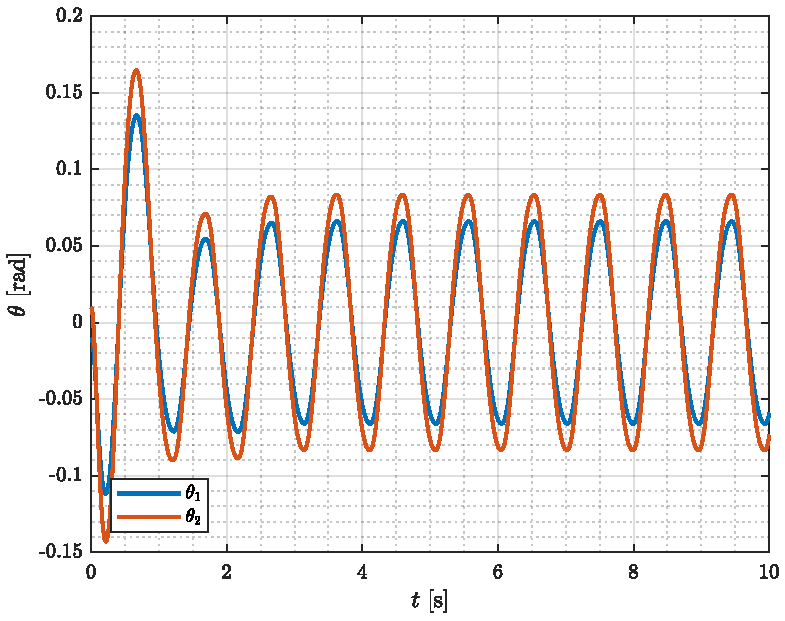
\includegraphics[width=.4\textwidth]{figures/theta_twinStabilize}
  }
  \hspace{20pt}
  \captionbox 
  {
    The cart position initially moves away from zero but returns to stabilize with some oscillations.
    \label{fig:x_twinStabilize}
  }
  {
    \hspace{-1cm}
    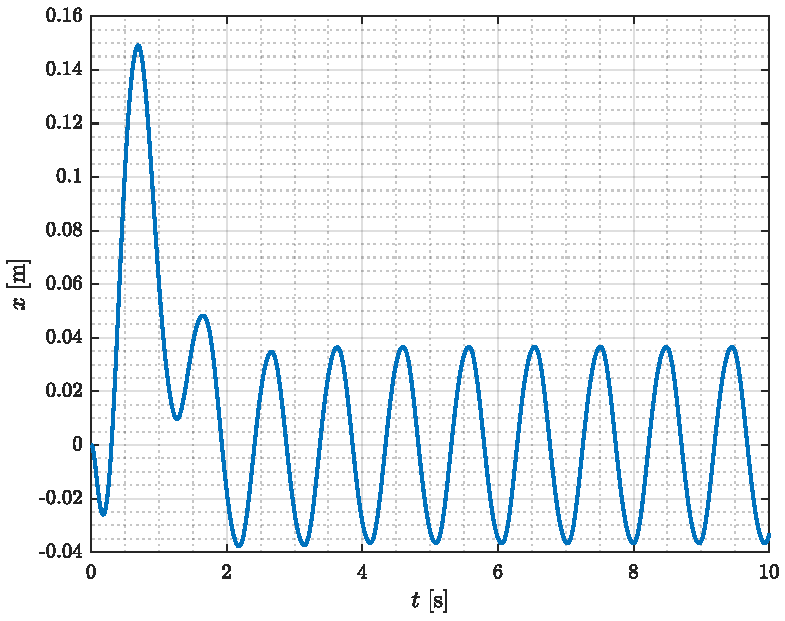
\includegraphics[width=.4\textwidth]{figures/x_twinStabilize}
  }  
\end{figure}
%
The required armature current for the LQR design is shown in \autoref{fig:ia_twinStabilize}, where the RMS current stays within the motor's maximum continuous current limit.
%
\begin{figure}[H]
  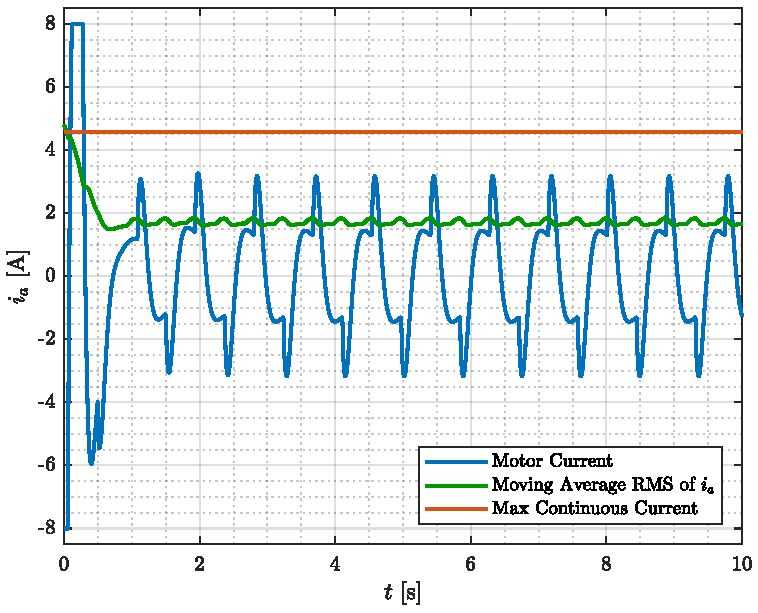
\includegraphics[width=.5\textwidth]{figures/ia_twinStabilize}
  \caption{The control signal required by the LQR design is considered reasonable with only short pulses exceeding the maximum continuous current rating of the motor.}
  \label{fig:ia_twinStabilize}
\end{figure}
%
With both the swing-up and stabilizing controller designed for the twin pendulum system, it is, in simulation, attempted to swing up and then catch both pendulums in upright position.\\
The swing-up controller bringing the pendulum energy errors to zero ensures convergence to the heteroclinic orbit of each pendulum. However, it does not promise timing such that both pendulums reach the equilibrium simultaneously. For this reason it is found necessary to split the tuning gain $k$ such that the new control law becomes,
\begin{align}
  G &= k_1 m_1 l_1 E_{\Delta_1} \cos \theta_1 \dot{\theta}_1 +  k_2 m_2 l_2 E_{\Delta_2} \cos \theta_2 \dot{\theta}_2  \label{eq:2k_lyapunovDerivativeTwinG} \\
  a_c &= sat( - G ) \ \ \ .  \label{eq:2k_twinSwingControl1}
\end{align}
%
It is further found useful to tune the energy reference of each pendulum separately. In the following simulations, see \autoref{fig:theta_twinSwingAndCatch} and \ref{fig:x_twinSwingAndCatch}, the energy reference of the first pendulum, $E_{\Delta_1}$, is increased by \SI{0.030}{J} and for the second pendulum $E_{\Delta_2}$ is increased by \SI{0.028}{J}. The gains are tuned to $k_1 = 25$ and $k_2 = 17$.
%
\begin{figure}[H]
  \hspace{-10pt}
  \captionbox 
  {
    A simulation of the twin pendulum using the energy based swing-up controller and catching with the LQR.
    \label{fig:theta_twinSwingAndCatch}
  }
  {
    \hspace{-1cm}
    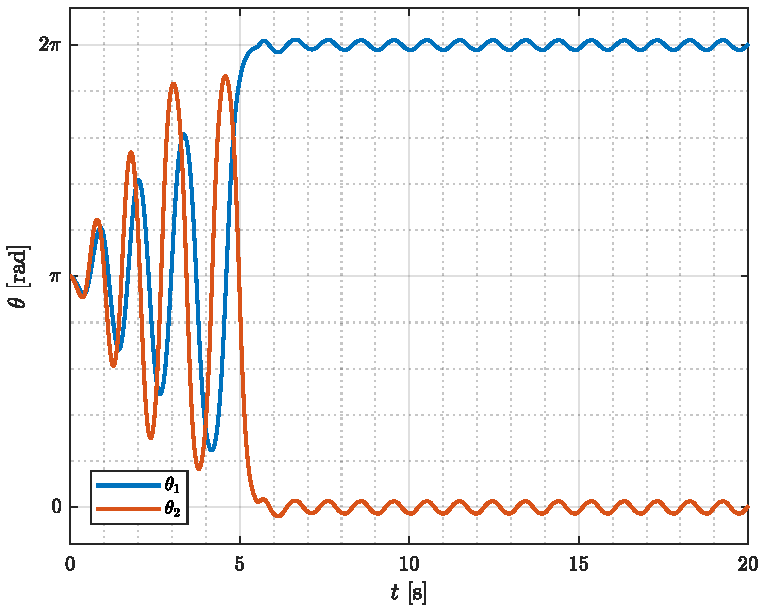
\includegraphics[width=.46\textwidth]{figures/theta_twinSwingAndCatch}
  }
  \hspace{20pt}
  \captionbox 
  {
    The $x$ position controller keeps the cart away from the rail edge while the swing-up controller approaches equilibrium.
    \label{fig:x_twinSwingAndCatch}
  }
  {
    \hspace{-1cm}
    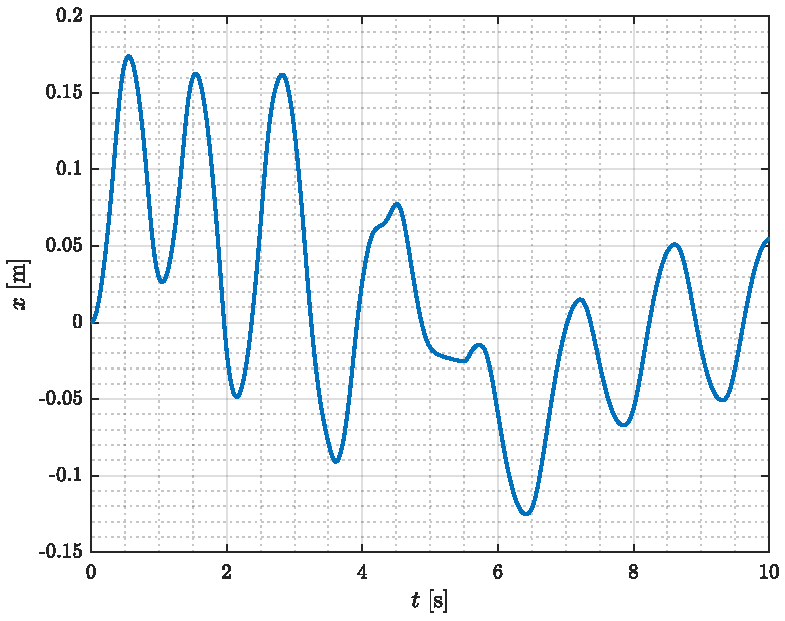
\includegraphics[width=.46\textwidth]{figures/x_twinSwingAndCatch}
  }
\end{figure}
%
The control signal used to obtain the result in \autoref{fig:theta_twinSwingAndCatch} and \ref{fig:x_twinSwingAndCatch} is shown in \autoref{fig:ia_twinSwingAndCatch}.
%
\begin{figure}[H]
  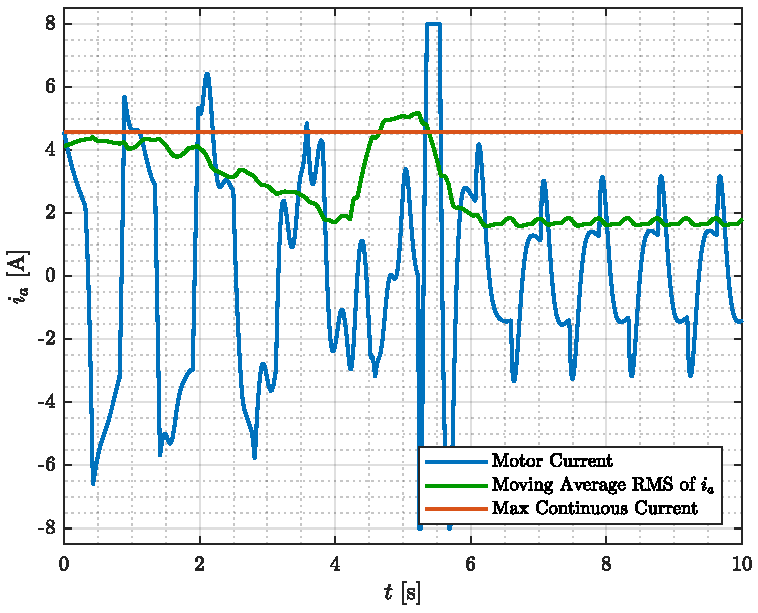
\includegraphics[width=.5\textwidth]{figures/ia_twinSwingAndCatch}
  \caption{The needed armature current for the simulated behavior of swing-up and catch.}
  \label{fig:ia_twinSwingAndCatch}
\end{figure}
%
%\begin{figure}[H]
%  \hspace{-10pt}
%  \captionbox
%  {
%    a
%    \label{fig:x_twinSwingAndCatch}
%  }
%  {
%    \hspace{-1cm}
%    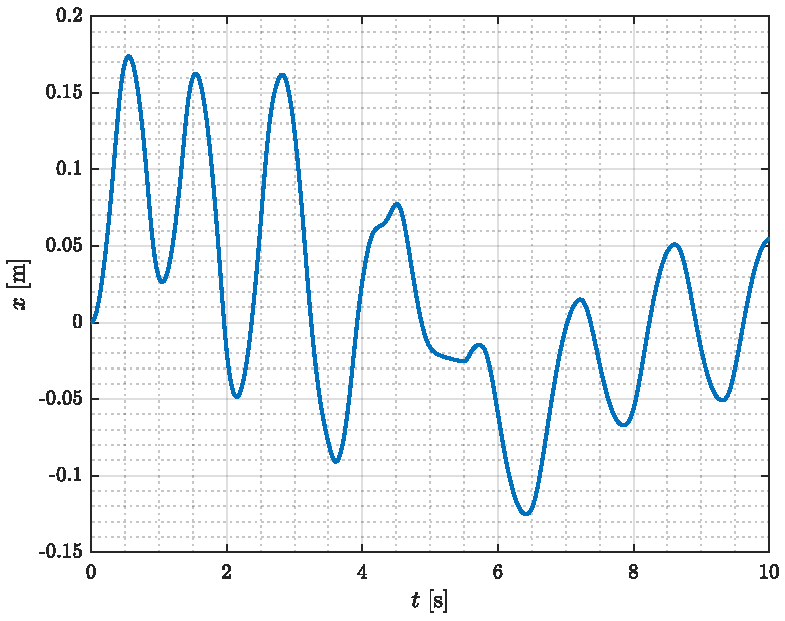
\includegraphics[width=.4\textwidth]{figures/x_twinSwingAndCatch}
%  }
%  \hspace{20pt}
%  \captionbox 
%  {
%    a
%    \label{fig:xDot_twinSwingAndCatch}
%  }
%  {
%    \hspace{-1cm}
%    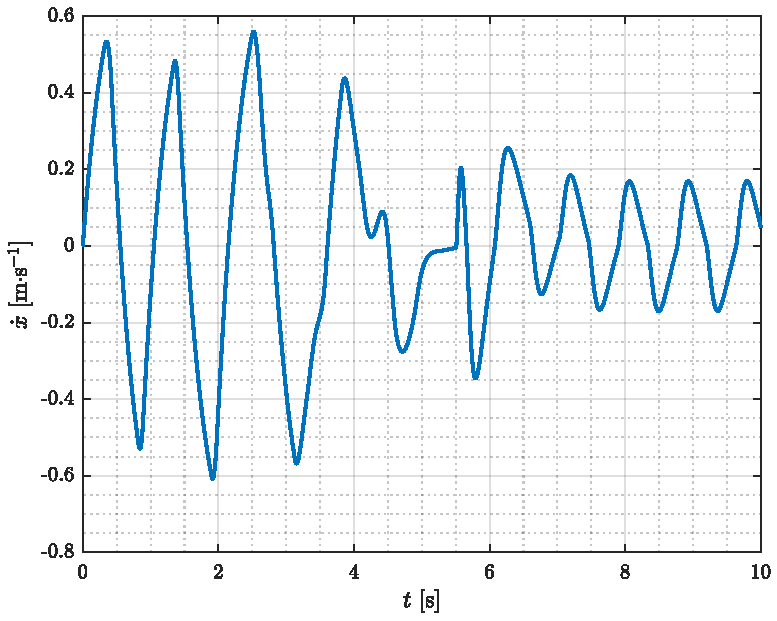
\includegraphics[width=.4\textwidth]{figures/xDot_twinSwingAndCatch}
%  }  
%\end{figure}
%
%
%\begin{figure}[H]
%  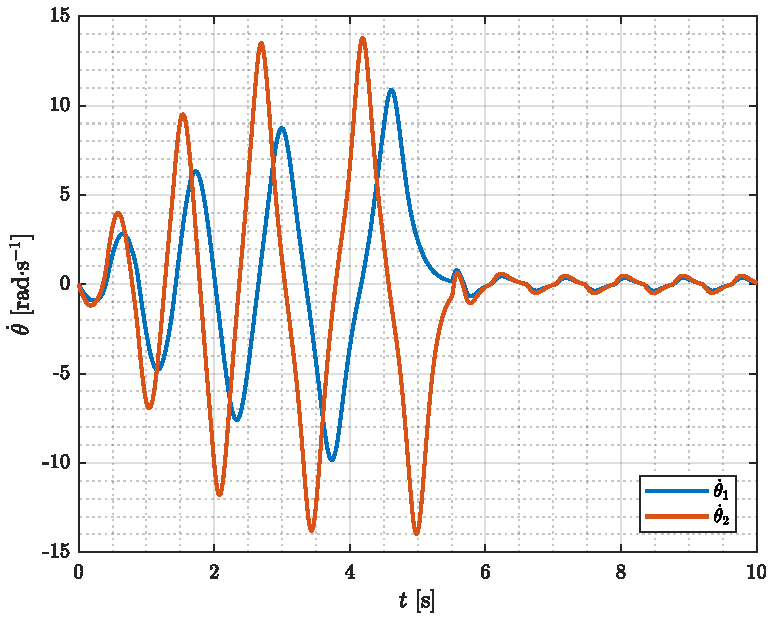
\includegraphics[width=.6\textwidth]{figures/thetaDot_twinSwingAndCatch}
%  \caption{thetaDotTwinSwingAndCatch}
%  \label{fig:thetaDot_twinSwingAndCatch}
%\end{figure}
%\begin{figure}[H]
%  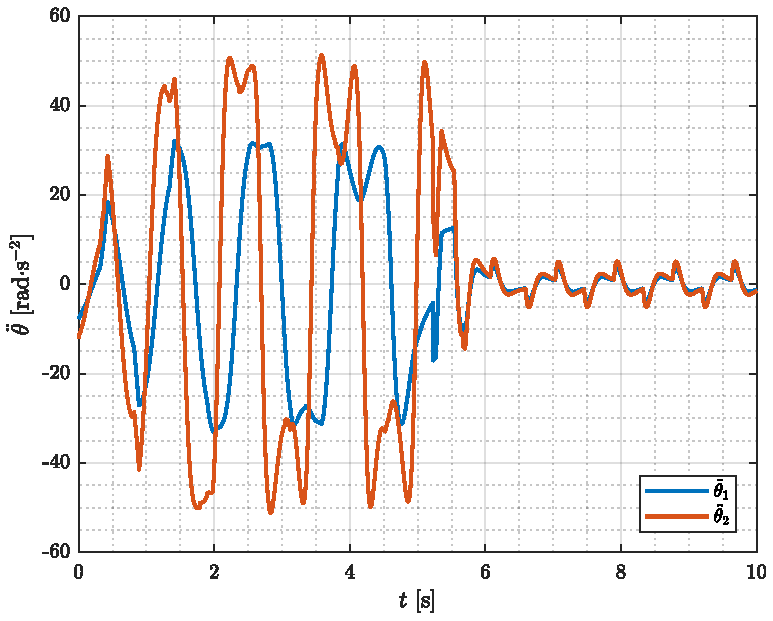
\includegraphics[width=.6\textwidth]{figures/thetaDotDot_twinSwingAndCatch}
%  \caption{thetaDotDotTwinSwingAndCatch}2.
%  \label{fig:thetaDotDot_twinSwingAndCatch}
%\end{figure}
%\begin{figure}[H]
%  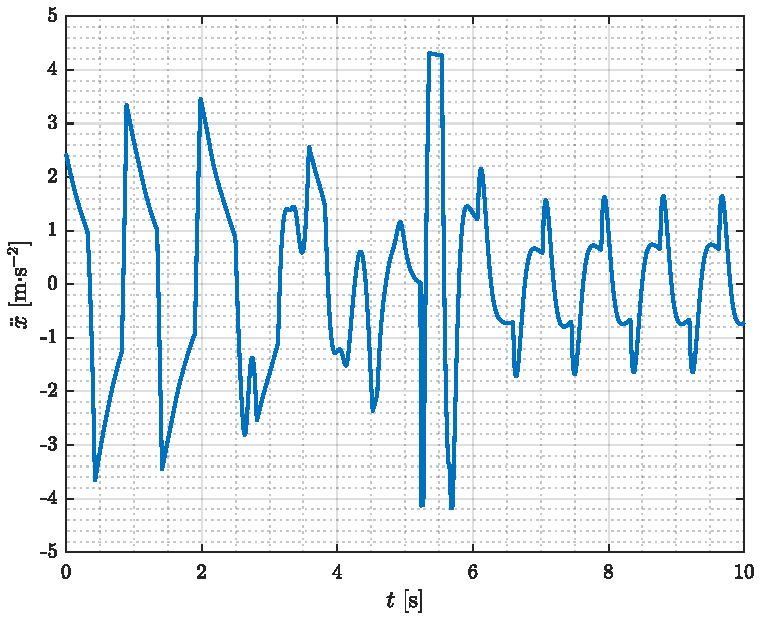
\includegraphics[width=.6\textwidth]{figures/xDotDot_twinSwingAndCatch}
%  \caption{xDotDotTwinSwingAndCatch}
%  \label{fig:xDotDot_twinSwingAndCatch}
%\end{figure}
%
%
%
%
The energy control strategy from \textit{Part 1} was successfully adapted as a swing-up controller for twin pendulum system. Further the swing-up controller was tuned to bring both pendulums into equilibrium at the same time for the LQR controller to catch both pendulums in simulation.\\
To implement the control strategies, the next chapter is concerned with estimating the three unmeasured states of the twin pendulum system.